\begin{frame}[allowframebreaks]{Problems with GANs}
\begin{itemize}
    \item Vanishing Gradients 
    \begin{itemize}
        \item When the discriminator is perfect, we are guaranteed with $D(x) = 1, \forall x \in p_{data}$ and $D(x) = 0, \forall x \in p_G$.
        \item The loss function drops to zero, resulting in no gradient for updates.
        \item \textbf{Solution}: Perform gradient ascent on the generator, i.e., use a different objective:
        $$\max_{\theta_G} E_{x \sim p(z)} log(D_{\theta_D}(G_{\theta_G}(z)))$$
    \end{itemize}
\end{itemize}

\framebreak

\begin{figure}
    \centering
    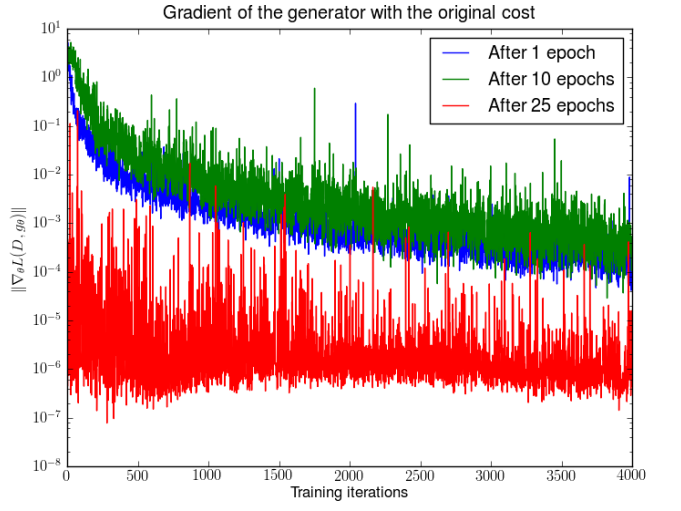
\includegraphics[height=0.8\textheight, width=\textwidth, keepaspectratio]{images/gan/gan_generator_gradient.png}
    \caption{Vanishing gradient in GANs (Image source: \href{https://arxiv.org/pdf/1701.04862.pdf}{Arjovsky and Bottou, 2017})}
\end{figure}

\framebreak

\begin{itemize}
    \item Difficulty in achieving Nash equilibrium
    \begin{itemize}
        \item GANs involve training two models simultaneously to reach a Nash equilibrium in a two-player non-cooperative game. However, since each model updates its cost independently, convergence is not guaranteed.
        \item For practical tips on training GANs, see "How to Train a GAN? Tips and tricks to make GANs work" by Soumith Chintala: \href{https://github.com/soumith/ganhacks}{https://github.com/soumith/ganhacks}
    \end{itemize}
\end{itemize}

\framebreak
\begin{itemize}
    \item Mode collapse
    \begin{itemize}
        \item The generator aims to fool the discriminator $D$ into classifying its outputs as real. If the generator $G$ finds a single output that consistently fools $D$, it may repeatedly produce that output, leading to mode collapse.
        \item Solutions to mode collapse are mostly empirical, including alternative architectures, modified GAN losses, and additional regularization terms.
        
        \begin{figure}
            \centering
            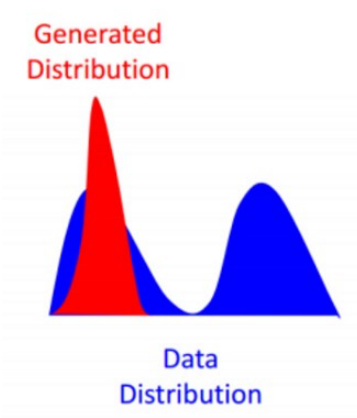
\includegraphics[height=0.4\textheight, width=\textwidth, keepaspectratio]{images/gan/gan_mode_collapse_1.png}
        \end{figure}
    \end{itemize}
\end{itemize}

\framebreak
\begin{figure}
    \centering
    
\includegraphics[height=0.85\textheight, width=\textwidth, keepaspectratio]{images/gan/gan_mode_collapse_2.png}
    \caption{GAN mode collapse on MNIST digits dataset}
\end{figure}
    
\end{frame}